% \documentclass[lineno,twocolumn,endfloat,biblatex]{biophys-new}
\documentclass{biophys-new}
\usepackage[utf8]{inputenc}
\usepackage{graphicx}
\usepackage[colorlinks,allcolors=cyan!70!black]{hyperref}

% uncomment if using biblatex
% \addbibresource{sample.bib}

\usepackage{lipsum}

\title{Understanding the Free Energy Landscape of Phase Separation in Lipid Bilayer using Weighted Ensemble Molecular Dynamics}
\runningtitle{All plots with long captions} %% For page header

\author[1]{Ashlin Poruthoor}
\author[1,*]{Alan Grossfield}
\runningauthor{Poruthoor and Grossfield} %% For page header

\affil[1]{University of Rochester Medical Center, Rochester, NY 14620}

\corrauthor[*]{alan\_grossfield@urmc.rochester.edu}

% \papertype{Letters}
\papertype{Article}
% \papertype{Computational Tools}


\begin{document}

\begin{frontmatter}
\begin{abstract}

Lorem ipsum dolor sit amet, consectetur adipiscing elit, sed do eiusmod tempor incididunt ut labore et dolore magna aliqua. Ut enim ad minim veniam, quis nostrud exercitation ullamco laboris nisi ut aliquip ex ea commodo consequat. Duis aute irure dolor in reprehenderit in voluptate velit esse cillum dolore eu fugiat nulla pariatur. Excepteur sint occaecat cupidatat non proident, sunt in culpa qui officia deserunt mollit anim id est laborum.

\end{abstract}

\begin{sigstatement}

Lorem ipsum dolor sit amet, consectetur adipiscing elit, sed do eiusmod tempor incididunt ut labore et dolore magna aliqua. Ut enim ad minim veniam, quis nostrud exercitation ullamco laboris nisi ut aliquip ex ea commodo consequat. Duis aute irure dolor in reprehenderit in voluptate velit esse cillum dolore eu fugiat nulla pariatur. Excepteur sint occaecat cupidatat non proident, sunt in culpa qui officia deserunt mollit anim id est laborum

\end{sigstatement}

\end{frontmatter}

\section*{Introduction}

This is a place holder article template for our future paper. For time being, I will be using this 
space to publish all the plots that are being generated as a part of the analysis.

\section*{Methods}

\subsection*{System details}

Here, we used three different ternary lipid bilayer systems to test the hypothesis:
1. As the main test system, we chose a lipid bilayer consisting of dipalmitoyl-phosphatidylcholine (DPPC), dilinoleyl-phosphatidylcholine
(DIPC), and Cholesterol (CHOL) which is known to phase separate in silico in a few microseconds \cite{Risselada2008,Schafer2010,Janosi2012,Doma2012,Jong2013,Liu2020,Su2020}.
2. As a positive control, we chose a lipid bilayer consisting of DPPC, diarachidonoyl-phosphatidylcholine (DAPC), and CHOL, known to phase separate relatively faster in silico in the order of a few hundreds of nanoseconds \cite{Lin2016,Lin2019,Davis2013a}.
3. As a negative control, we chose a lipid bilayer consisting of DPPC, palmitoyl-oleoyl-phosphatidylcholine (POPC), and CHOL that was previously shown not to
phase separate \cite{Veatch2003,Davis2013a}.
The composition of DPPC-DIPC-CHOL, DPPC-DAPC-CHOL, and DPPC-POPC-CHOL systems used here are (0.42/0.28/0.3),
(0.5/0.3/0.2) and (0.4/0.4/0.2) respectively and were adapted from previous studies \cite{Risselada2008,Lin2016,Davis2013a}.

Due to the relatively larger system size and time scale required for phase separation and related dynamics in lipid bilayer simulations, the Coarse-Grained (CG) model of 
each system was used.
Hence the subsequent dynamics propagation using MD is relatively cheaper than an All-Atom model but with the tradeoff in system resolution.
The rationale behind this design choice is to fail faster with minimum resources if this proof-of-concept protocol is not working as expected. 
Using CHARMM-GUI Martini Maker \cite{Qi2015}, we constructed four random replicas of each CG ternary symmetric bilayer system.
MARTINI 2 force field parameters and particle definitions were used to construct CG systems and to run the subsequent MD simulation. 
The default input files from CHARMM-GUI Martini Maker were replaced with their respective most recent Martini 2.x versions, if they existed.
MARTINI polarizable water model was used to solvate all systems with approximately a 1:30 lipid to real water ratio.
A detailed description of the systems used can be found in the Table S1 of supplementary material.

\subsection*{Standard MD simulation details}

Due to the historical compatibility of the the GROMACS MD engine with the MARTINI force field, we used GROMACS 2020.3 to propagate the dynamics of the systems prepared. 
Each system was minimized and equilibrated in steps using the MD input files suggested by CHARMM-GUI Martini Maker.

To obtain an intact bilayer without any membrane undulations, we used an additional membrane restraining protocol: 
We took advantage of the flat bottom restrain potential available in GROMACS to allow lipids to move freely in the $xy$ plane but restrained within a slab of
defined z thickness.
More details about membrane restraining protocol can be found in the supplementary material.

After the minimization and equilibration, all systems were run at 400 K in the NPT ensemble for 100 ns to make sure the lipids in each system were
randomly distributed.
For every system, each replica was then forked into multiple temperature runs. 
For the positive control, DPPC-DAPC-CHOL lipid bilayer system, every replica was simulated at 298 K, 323 K, 333 K, 343 K, 353 K, 373 K, 423 K and, 450 K. 
For the main test system, DPPC-DIPC-CHOL lipid bilayer, every replica was simulated at 298 K, 323 K, 333 K, 343 K, 353 K, 423 K, and 450 K. 
For the negative control, DPPC-POPC-CHOL lipid bilayer system, every replica was simulated at 298 K, 323 K, and 450 K.
All standard MD simulations were run for at least 8 microseconds using the BlueHive supercomputing cluster of the Center for Integrated Research and
Computing at the University of Rochester. Simulations were run on Intel Xeon E5-2695 and Gold 6130 processors augmented with Tesla K20Xm, K80, and V100 GPUs.   
The trajectories were processed and analyzed using LOOS software package.
A detailed description of the simulation parameters can be found in the Table S1 of supplementary material.  

\subsection*{Collective Variable}

A collective variable (or a set of variables) is a reduced coordinate that captures the progress of a system along the transition of interest.
Ideally, such a reduced variable(s) should capture the key slow modes of transition to reflect the complex event under study fully.
The success of any enhanced sampling protocol depends on the chosen collective variable over which the sampling is enhanced. 
In our case, phase separation in a lipid bilayer is characterized by the formation of lipid domains with distinct properties from the rest of the bilayer.
Hence we hypothesized that a variable that quantifies the recruitment of lipids into such domains could be used to track the phase separation
events in our systems. Here, we define the Fraction of Lipids in Cluster (FLC) as follows:

\begin{equation}
\label{eq:CLT}
\text{FLC} = \sum_{i}^{N} \frac{\text{No. of Lipid $X_i$ in Lipid $X_i$ Clusters}}{\text{No. of Lipid $X_i$}} =  \frac{\sum_{i}^{N} \text{No. of Lipid X$_i$ in Lipid X$_i$ Clusters}}{\text{Total No. of Lipids}}
\end{equation}


Where subscript $i$ denotes the individual lipid species in a bilayer consisting of N total lipid species.
As shown in Figure \ref{fig1:view}, each system has $N=3$ lipid species in our case.
FLC increases as the system go from a mixed state, with a random distribution of lipids, to a separated state.
In principle, FLC is bounded between 0 and 1. FLC = 0 corresponds to a system configuration where no lipids are part of any cluster.
While FLC = 1 corresponds to all lipids being a part of some cluster. 
However, the actual bound of FLC will be a function of system composition and interactions.

\begin{figure}[hbt!]
\centering
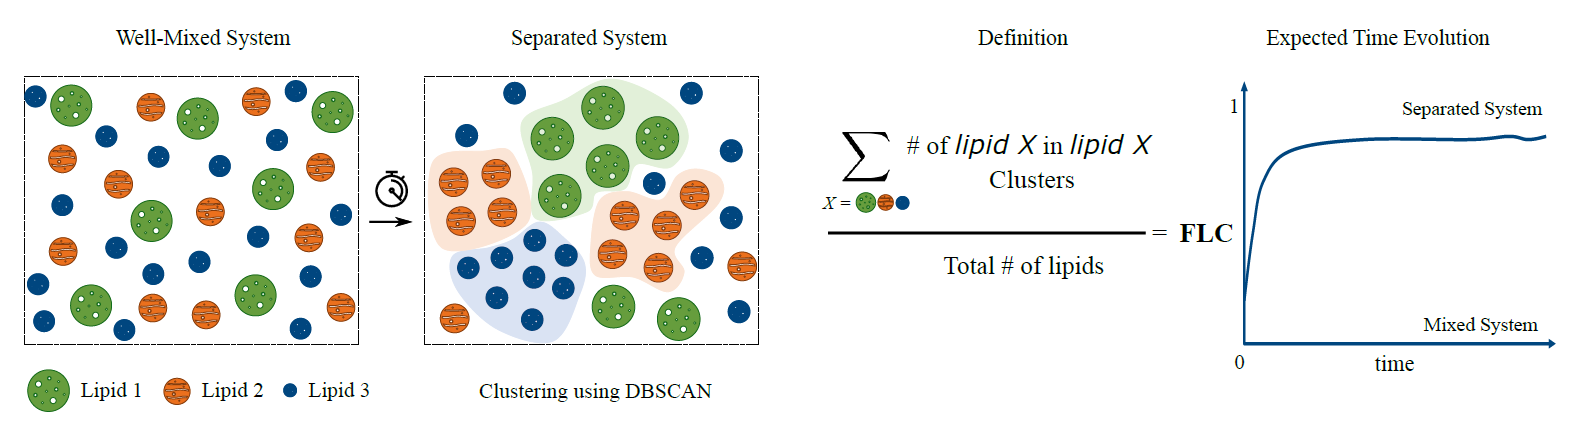
\includegraphics[width=1\linewidth]{Figures/Figure1.PNG}
\caption{a. A phase separating system evolves from a mixed state to a separated state. b. Functional form of FLC. c. FLC evolution curve for a phase separating system}
\label{fig1:view}

\end{figure}


The lipid $X_i$ cluster is defined using the Density-Based Spatial Clustering of Applications with Noise (DBSCAN) algorithm \cite{MartinEsterHans-PeterKriegelJiirgSander1996,Ester2017} as implemented in scikit-learn \cite{PedregosaF.VaroquauxG.GramfortA.MichelV.ThirionB.GriselO.BlondelM.PrettenhoferP.WeissR.andDubourgV.VanderplasJ.PassosA.CournapeauD.BrucherM.PerrotM.Duchesnay2011}.
For lipid DBSCAN clustering, instead of the default euclidean metric to calculate the distance between lipid coordinates, we used a precomputed distance matrix adjusted for periodic boundary conditions of the simulation box using LOOS.
Two additional input parameters are required by the algorithm: $min\_samples$ and $\varepsilon$.
Lipids with more than $min\_samples$ neighbors (including the lipid itself) within $\varepsilon$ radius are considered as core lipids.
Non-core lipids that are still within $\varepsilon$ radius of a core lipid are considered border lipids.
A set of core lipids within $\varepsilon$ radius of each other and their border lipids forms a cluster.
All lipids that are not a part of any cluster are considered outlier lipids.

Since lipid motion in a bilayer is predominantly constrained in a plane and MARTINI beads for a lipid are of similar radii, we can make use of the two-dimensional
version of Kepler's conjecture that the densest packing of unit disks in a plane is hexagonal close packing (Thue's Theorem).
Hence we chose 7 (6 nearest neighbors + 1 central lipid) as $min\_samples$ for all the lipid species.

However, $\varepsilon$ was chosen differently for each lipid species based on their first nearest neighbor distance from the central lipid.
The first nearest neighbor distance of an individual lipid species was calculated using the $xy\_rdf$ tool in LOOS.
From the first 8 $\mu$s MD standard simulation of each replica, we computed the radial distribution function (RDF) for a lipid species in the xy-plane. 
From the RDF plot, we found the first maxima (provided it is above 1), and the distance to the minima right after this first maxima were determined to be the first nearest neighbor distance for that lipid species.
This distance was averaged over all four replicas for a given system at a given temperature and was assigned as the respective $\varepsilon$ input.
Since nearest neighbor distance is a function of temperature, for the same lipid species in the same system, $\varepsilon$ may be different for different temperatures.
Computed $\varepsilon$, i.e., average first nearest neighbor distance for different conditions are plotted in Supplementary Figure S1.

\subsection*{Auxiliary Variables}

Additional auxiliary variables (AVs) were tracked parallel to the primary collective variable, FLC. 
Following are the definitions of AVs that evaluate the quality of DBSCAN clustering since it is critical for defining the FLC that drives the WE equilibrium dynamics. 
For each $X_i$ lipid species in the system, we calculated the following, 

1. Number of $X_i$ clusters in the system under study.

2. Fraction of $X_i$ lipids in $X_i$ clusters

3. Fraction of $X_i$ lipids in $X_i$ core lipids.

4. Fraction of outliers in the system.

5. Mean Silhouette Coefficient (MSC) of $X_i$ Clusters, as implemented in scikit-learn.

Silhouette Coefficient is a method used to evaluate the clustering done by any technique, especially if ground truth labels are unknown. 
Here, for a $X_i$ lipid in the cluster, mean intra-cluster distance (a) from other $X_i$ lipids in the cluster is found.  
Similarly, for a $X_i$ lipid in the cluster, the mean nearest-cluster distance (b) is also calculated.
While the former assesses the 'cohesion' of a given $X_i$ lipids with other $X_1$ lipids in a cluster, the latter assesses the 'separation' from the nearest cluster.
Thus, Silhouette Coefficient for a $X_i$ lipid, s, is defined as below,

\begin{equation}
\label{eq:SC}
\text{s} = \frac{b - a}{max(a,b)}
\end{equation}

The Mean Silhouette Coefficient of $X_i$ Clusters is given by the mean $s$ over all non-outlier $X_i$ lipids.
Here, we have omitted the MSC calculations for cases when there are no clusters or just one cluster detected by DBSCAN. 
MSC is bound between and -1 and 1.
A high positive value corresponds to well segregated dense clusters, while a low negative value implies that lipids are assigned to clusters incorrectly.  

Following are the definitions of another set of AVs similar to FLC that can track phase separation and serves to assess phase separation events enhanced by FLC driven WE runs.

1. Cumulative Enrichment Index (CEI)

2. Segregation Index (SI)

3. Weighted Mean Lipids in Clusters Vs. Weighted Standard Deviation of Lipids in Clusters

4. Hexactic Order Parameter (HOP)

5. Area swept by Nearest Neighbors (ANN) with respect to ideal Hexagonal Closed Packing Area

6. Chain Entropy of lipid tails

7. FLC defined using Support Vector Machine (SVM) instead of DBSCAN.

\subsection*{Weighted Ensemble Simulation}

\textbf{Preparing seeding configurations for WE simulation:} 
From each 8 $\mu$s replica MD simulation of a given system, the last 10 frames spaced by 100 ns were collected.
Using such collected frames, for each replica of a given system, we created sets of mixed and separated configurations for each replica of a given system.
For DPPC-DAPC-CHOL and DPPC-DIPC-CHOL systems, the set of mixed configurations for a particular replica came from the respective 423 K and 450 K simulation frames. 
While the set of separated configurations for a replica came from  the respective 298K and 323K simulation frames.
For the DPPC-POPC-CHOL system, sets of mixed and separated configurations for a replica came from the 450 K and 298K simulation frames respectively.
To enhance the convergence of WE equilibrium simulations, we decided to seed each simulation from both mixed and separated states and let the enhanced sampling cover the transition between them.

\textbf{Running WE simulations:} 
Weighted Ensemble equilibrium simulations were run using the WESTPA 1.0 software package.
The collective variable was divided into 30 dynamic bins using the minimal adaptive binning scheme (MAB).
For each replica, a target number of 4 short simulations, or "walkers" per bin, were started in parallel from the mixed and the separated configurations prepared earlier.
After every resampling interval of 1 ns, the collective variable was evaluated to initiate the merging and splitting of walkers to maintain the target number of walkers per bin.
A short 1 ns MD run of all the walkers and subsequent resampling, according to the standard WE algorithm, constituted 1 WE iteration. 
We conducted 500 WE iterations for each replica.
The MD propagation was done using GROMACS 2020.3 engine with the same parameters used for standard MD simulations described earlier.
A WE Equilibrium Dynamics (WEED) reweighting protocol, implemented in WESTPA 1.0, was used to accelerate the convergence of WE walkers into an equilibrium. 

The reweighting was done every 10 WE iterations.

For the DPPC-DAPC-CHOL lipid bilayer system, four WE replicas were simulated at 298 K, 323 K, 333 K, 343 K, 353 K, 373 K, and 423 K. 
For the DPPC-DIPC-CHOL lipid bilayer system, four WE replicas were simulated at 298 K, 323 K, 353 K, and 450 K. 
For the DPPC-POPC-CHOL lipid bilayer system, four WE replicas were simulated at 298 K and 450 K.
All WE runs were carried out using the Intel Xeon E5-2695 and Tesla K20Xm GPUs in the BlueHive supercomputing cluster of the Center for Integrated Research and
Computing at the University of Rochester.   

\textbf{Analysis of WE simulations:}
The probability distribution of CV and AVs for each replica, as a function of WE iterations, was constructed using $w\_pdist$ and $plothist$ tools in WESTPA.
Using this distribution, we monitored the evolution of each WE replica simulation and the convergence.
$w\_mult\_west$ tool in WESTPA was used to combine data from four WE replicas of a system at a given temperature.
From the combined probability distribution of a system, the respective Free Energy Surface (FES) was created.
To check the flux between states and population in different states, $w\_ipa$, another WESTPA tool, was used.
For 



\section*{Results}

[] CV makes sense as we see CV track phase separation in vanilla sims.
Plot CV evolution of vanilla simulation for each system - Will go in supplementary material

[] If time permits, When plotting FES for auxillary variables, add a plot for FES as a function of border lipids as well.
Might need to use $w_crawl$ and add an extra lines of code to print out border lipid number in FLC script.


% ------------------------- %
% Uncomment if using bibtex (default)
\bibliography{Academics-Grossfield_lab-Phase_Seperation}

\end{document}